\chapter{System Design}

\section{Architectural Overview}

Anhoc uses a three-tier web architecture. A Next.js frontend provides the user interface. An Express backend exposes REST endpoints and business logic. PostgreSQL stores content, user identities, generated snapshots, and progression data. Prisma acts as the ORM boundary between the backend and the database.

\begin{figure}[H]
\centering
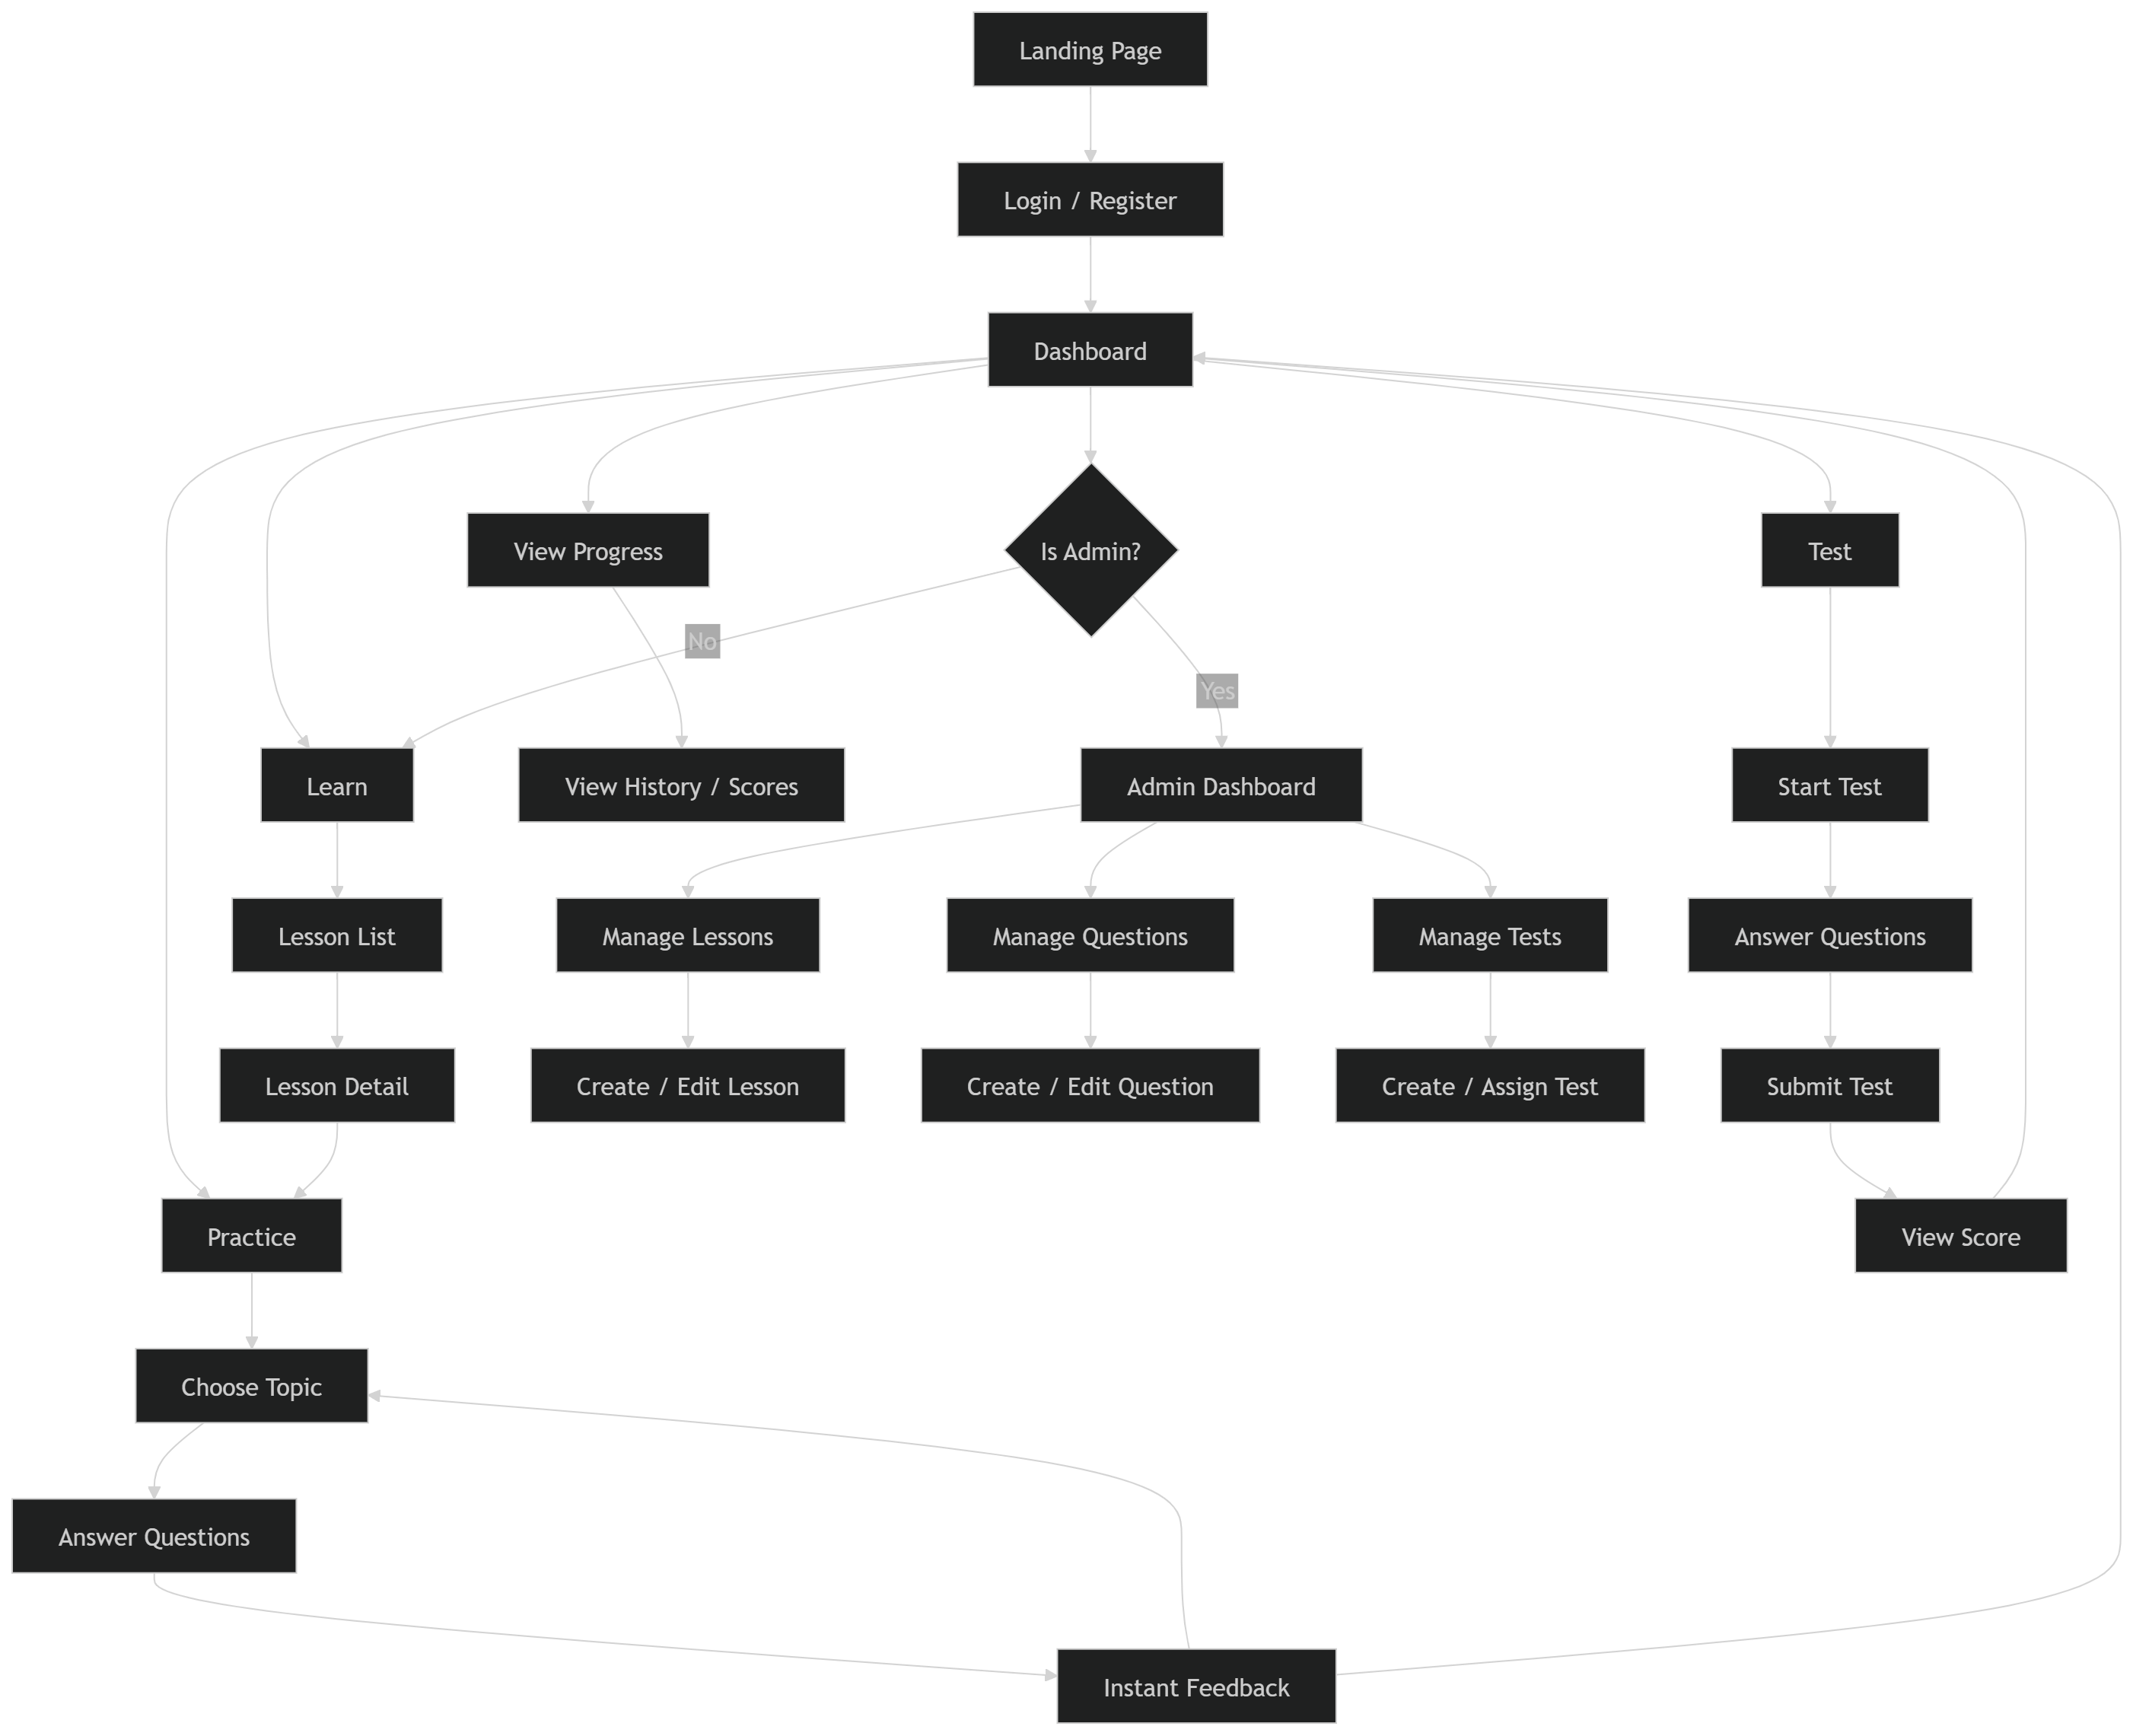
\includegraphics[width=0.9\textwidth]{../../images/anhoc-user-flow.png}
\caption{User-facing flow of the Anhoc platform}
\label{fig:user-flow}
\end{figure}

At a high level, the request flow is:
\begin{enumerate}
  \item the browser interacts with the Next.js frontend;
  \item the frontend calls backend routes under \code{/api/v1};
  \item the backend validates identity and permissions;
  \item business services coordinate data access and progression updates;
  \item PostgreSQL persists authoritative state.
\end{enumerate}

\section{Deployment Design}

The repository documents a practical deployment split:
\begin{itemize}
  \item Vercel hosts the frontend runtime;
  \item Render hosts the Node.js API;
  \item Neon provides PostgreSQL infrastructure.
\end{itemize}

This split is appropriate for a full-stack TypeScript project because it separates the static or server-rendered frontend from the API runtime and keeps the relational database independent of either application tier.

\section{Backend Design}

The backend entry point is \code{backend/server.ts}. It initializes Express, configures CORS, enables JSON parsing, mounts route modules, exposes a health endpoint, and conditionally seeds achievements at startup. The route structure is organized by domain:

\begin{itemize}
  \item \code{auth.ts} for identity, login, and profile operations;
  \item \code{lessons.ts} for educational content and practice initiation;
  \item \code{tests.ts} for attempts, answer submission, template management, and reports;
  \item \code{admin.ts} for users, roles, access control, and statistics;
  \item \code{achievements.ts} for achievement retrieval and re-evaluation.
\end{itemize}

This separation keeps HTTP concerns close to route boundaries while pushing calculation-heavy logic into services.

\section{Frontend Design}

The frontend is built with Next.js using an app-router structure under \code{frontend/src/app}. It includes separate areas for authentication, student flows, and administration. The frontend is supported by Axios-based service modules, Redux state for authentication and permissions, and feature-specific components such as lesson cards, question players, result modals, and achievement galleries.

From a design perspective, the frontend acts as an orchestration layer:
\begin{itemize}
  \item it collects user input and triggers backend operations;
  \item it renders lesson, practice, test, and admin views;
  \item it persists authentication tokens in browser storage and cookies;
  \item it enforces route-level and component-level access decisions using the permission payload returned by the backend.
\end{itemize}

\section{Security Model}

Authentication is handled with JWT bearer tokens. The middleware in \code{backend/middleware/auth.ts} extracts the token from the \code{Authorization} header, verifies it using the configured secret, and attaches the decoded payload to the request object.

Authorization is layered on top of authentication. The project uses:
\begin{itemize}
  \item role identity for coarse-grained decisions;
  \item grouped resource permissions for action checks;
  \item subject-level role restrictions for scoped access;
  \item helper middleware such as \code{isAdmin} and \code{selfOrAdmin}.
\end{itemize}

The design choice to keep permissions data-driven is significant. It allows new resources and actions to be introduced through database records and route logic instead of forcing the codebase into a rigid two-role system.

\section{Data Model}

The database schema in \code{backend/prisma/schema.prisma} defines the educational, assessment, and progression domain. Table \ref{tab:main-entities} summarizes the most important entities.

\begin{longtable}{L{0.28\textwidth}L{0.62\textwidth}}
\caption{Main persistent entities}\label{tab:main-entities}\\
\toprule
\textbf{Entity} & \textbf{Purpose} \\
\midrule
\endfirsthead
\toprule
\textbf{Entity} & \textbf{Purpose} \\
\midrule
\endhead
\code{users} & Stores account identity and links to roles, attempts, mastery, achievements, and statistics. \\
\code{roles}, \code{actions}, \code{resources}, \code{role\_permissions} & Implements dynamic role-based access control. \\
\code{subjects}, \code{grades}, \code{lessons} & Represents the educational content hierarchy. \\
\code{question\_templates} & Stores reusable question definitions and logic. \\
\code{test\_attempts} & Stores headers for practice and test sessions. \\
\code{question\_snapshots} & Stores concrete generated questions bound to attempts. \\
\code{user\_lesson\_mastery} & Stores lesson-level progress and completion status. \\
\code{student\_stats}, \code{xp\_logs} & Stores aggregate progression state and XP history. \\
\code{achievements}, \code{user\_achievements} & Stores gamification rewards and earned records. \\
\code{question\_template\_reports} & Stores reports for problematic questions. \\
\code{audit\_logs}, \code{activity\_evidence} & Supports traceability and evidence collection. \\
\bottomrule
\end{longtable}

\section{Question Snapshot Strategy}

One of the strongest design decisions in Anhoc is the separation between \code{question\_templates} and \code{question\_snapshots}. Templates describe how a question can be generated. Snapshots record the exact generated variables, accepted answers, student response, correctness result, and awarded points for one attempt.

This decision solves several engineering problems:
\begin{itemize}
  \item a generated question does not change after the student starts an attempt;
  \item grading can be reproduced later without regenerating random variables;
  \item question reporting can refer to a concrete faulty instance rather than an abstract template;
  \item analytics can distinguish between template quality and attempt outcomes.
\end{itemize}

\section{Progression Design}

Progression in Anhoc is not limited to a final score. The backend updates several layers of state:
\begin{itemize}
  \item lesson mastery based on lesson-linked practice results;
  \item XP logs for additive progression history;
  \item aggregate student statistics for dashboards and profile displays;
  \item achievements that can also grant extra XP.
\end{itemize}

This design supports both immediate feedback and longitudinal tracking, which is more appropriate for learning software than a simple pass or fail test history.
